% ---------------------------------------------------------------------------
% Section fragment: execution failure and re-entrant recovery (domain: recovery)
% Sources: W/repo/htn-biology at commit 61d18d8. Figures in figures/recovery/.
% ---------------------------------------------------------------------------
\section{Execution Failure and Re-entrant Recovery with IPyHOP}
\label{sec:recovery}

The Checkpoint~2 report treats web construction as an offline planning problem: the planner returns a
primitive action sequence and the only notion of failure is a method that cannot be refined, after which
``the planner backtracks to the next method'' (its Algorithm~1). A spider that is \emph{executing} that
sequence faces a different problem. An attachment can miss, an anchor point can turn out to be unusable,
a route along existing threads can be blocked, a thread that was already laid can lose its support, and
silk can run short. In each case real time, travel and silk have already been spent, the spider is
wherever the failed action left it, and some already-planned later work may now be wrong. This section
documents the repository's work on that problem: a separate recovery benchmark built around the published
re-entrant HTN planner IPyHOP~\cite{bansod2021reentrant,bansod2022middle}, its later integration into the
Mulder moving-support model (``v4''), and an audit of which search strategy the planner actually used.
None of this material is in the Checkpoint~2 report, and part of it corrects that report.

Following the repository's review (\texttt{docs/research/BANSOD\_REENTRANT\_REVIEW.md}) we keep three
meanings of ``going back'' apart:
\begin{enumerate}
  \item \textbf{search backtracking}: abandoning a hypothetical method choice \emph{during planning};
        nothing physical has happened;
  \item \textbf{execution recovery}: revising unfinished work from \emph{observations} after a real action
        failed; time, travel, partial effects and position are not undone;
  \item \textbf{physical retracing}: actually walking back along existing threads, which needs explicit
        traversal actions and reachability; neither search backtracking nor re-entrancy provides it by
        itself.
\end{enumerate}

% ---------------------------------------------------------------------------
\subsection{Correction: the planner that was run does not backtrack}
\label{sec:recovery-strategy}

Section~2 of the Checkpoint~2 report describes the underlying planner as ``GTPyhop-style total-order
forward decomposition with chronological backtracking'', and its Algorithm~1 loops over all methods of a
compound task, trying the next method whenever the recursive call on the current one returns
\textsc{Fail}. The text after Algorithm~1, Section~3.3 and the caption of Algorithm~4 attribute the
model's proto-hub ``opportunism'' to this backtracking, and the conclusion repeats it. The repository's
planner-strategy audit (\texttt{docs/research/probes/planner\_strategy.py}, result in
\texttt{docs/research/evidence/planner\_strategy\_audit.json}, ledger claims C15 and C22, and the caveat at
the top of the repository \texttt{README.md}) found the following.

\begin{itemize}
  \item The installed and now pinned GTPyhop~1.9.7 (\texttt{requirements.txt}) uses
        \texttt{seek\_plan\_iterative} by default. The package's own documentation describes this
        strategy as iterative greedy search with irrevocable commitment to the first \emph{applicable}
        method and no backtracking. Full backtracking exists as a separate option
        (\texttt{set\_recursive\_planning("iterative\_dfs\_backtracking")}, or the recursive DFS).
  \item No historical runner selects a strategy. We checked this for the code behind the Checkpoint~2
        report as well: \texttt{spider\_web\_htn/main.py} calls \texttt{gtpyhop.find\_plan} without setting
        one, and outside the new recovery package and the audit probes no repository file calls
        \texttt{set\_recursive\_planning}.
  \item A toy probe separates the two behaviours (Table~\ref{tab:recovery-audit}). Task \texttt{complete}
        has two methods. The first is applicable but expands to an action that always fails; the second
        succeeds. Under the default strategy \texttt{find\_plan} returns \texttt{False} after calling only
        the first method. Under explicit iterative DFS backtracking it calls both and returns
        \texttt{[(finish,)]}. We re-ran the probe at commit \texttt{61d18d8} and got identical
        observations and the same engine source hash.
\end{itemize}

\begin{table}[H]
\centering
\caption{Planner-strategy audit with GTPyhop 1.9.7 (engine source SHA-256 \texttt{394cc942\ldots}).
The first method is applicable but has an impossible descendant, and the second succeeds. We re-ran the
audit at commit \texttt{61d18d8} with identical output.\\ Source:
\texttt{docs/research/evidence/planner\_strategy\_audit.json}.}
\label{tab:recovery-audit}
\small
\begin{tabularx}{\linewidth}{@{}l>{\raggedright\arraybackslash}X>{\raggedright\arraybackslash}Xl@{}}
\toprule
Configuration & Strategy function & Methods called & Result \\
\midrule
installed default & \texttt{seek\_plan\_iterative} & \texttt{first\_method} & \texttt{False} \\
explicit DFS backtracking & \texttt{seek\_plan\_iterative\_} \texttt{backtracking} & \texttt{first\_method}, \texttt{second\_method} & \texttt{[(finish,)]} \\
\bottomrule
\end{tabularx}
\end{table}

\paragraph{What this means for the Checkpoint~2 description.} Algorithm~1 is a correct description of
DFS with chronological backtracking. It is not the behaviour of the planner as configured under the
pinned dependency. Under the default strategy a later method of a task is tried only when the earlier
methods are inapplicable \emph{at the point of choice} (they return $\bot$ immediately). It is not tried
after a failure further down. Two qualifications apply. First, the GTPyhop version installed when the
Checkpoint~2 report was compiled was not recorded: the first commit required only
\texttt{gtpyhop>=1.9.0}, and 1.9.7 was pinned on 2026-10-20, after the report. Second, the plan
visualised in that report is unaffected, because the report itself notes that backtracking never
triggered: the first alternative succeeded for every task, and greedy and backtracking search return the
same plan in that case. What does not hold is the claim that a downstream failure of
\textsc{Establish-Proto-Hub-Via-Walk} would make the planner fall back to the drop or Tarzan variants.
Following claim C15, we do not relabel the historical runs as DFS results either. Their search
completeness and any method-comparison claims are simply not established.

\paragraph{What the new baselines pin.} The GTPyhop baselines of the recovery benchmark
(\texttt{fresh\_root}, \texttt{component}) explicitly select \texttt{iterative\_dfs\_backtracking} and
restore the previous global strategy after each call. A test checks this
(\texttt{test\_strategy\_is\_restored\_after\_fresh\_search}), and the run's \texttt{provenance.json}
records \texttt{fresh\_strategy = iterative\_dfs\_backtracking} (claim C22). The Mulder~v4
\texttt{legacy} back-end and the whole-suffix control of Section~\ref{sec:recovery-v4} deliberately keep
the historical default, which \texttt{metadata.json} records as \texttt{legacy\_strategy =
seek\_plan\_iterative}. Their results must be read with that label.

% ---------------------------------------------------------------------------
\subsection{Recovery formulation}
\label{sec:recovery-formulation}

\subsubsection{Retained solution trees and re-entry}
IPyHOP~\cite{bansod2021reentrant} keeps the whole \emph{solution tree} rather than only the primitive
plan. Each node records its task or action, a status, a tag (\texttt{old}/\texttt{new}), the selected
method and an iterator over the methods not yet tried. The repository vendors the unmodified upstream
source (revision \texttt{bdda210}, BSD-3-Clause, per-file hashes in
\texttt{third\_party/IPyHOP/UPSTREAM.json}; the adapter refuses to run if another \texttt{ipyhop} shadows
it). A call \texttt{replan}$(s_{\mathrm{obs}}, n_f)$ with the observed state and the failed leaf $n_f$
does three things.
\begin{enumerate}
  \item It visits every node after $n_f$ in depth-first pre-order, reopens it and strips the refinement
        of every compound node. This is the conservative suffix invalidation of Bansod et al.'s
        Algorithm~3, not a minimal causal-dependency computation. Completed prefix nodes are re-tagged
        \texttt{old}.
  \item It backtracks from the parent of $n_f$ to the nearest completed compound node, drops that node's
        refinement and resumes its method iterator, so the \emph{next untried} method is used. If none
        remains, backtracking continues upward. If the root is exhausted, the tree is reduced to the root
        and the plan is empty.
  \item Planning resumes on the modified tree, and the actor executes the leaves tagged \texttt{new}, in
        depth-first order.
\end{enumerate}
Because methods already tried are not retried, the domain supplies a second, identical routing method
(\texttt{travel\_recompute}). After re-entry it gives an untried refinement that recomputes the route
against the newly observed edges. This is an explicit, equally shared domain-engineering choice, not a
learned method generator.

\subsubsection{The sector-construction domain}
The benchmark (\texttt{spider\_web\_recovery/domain.py}) is a deliberately small abstraction, not the
Mulder geometry. It has a hub, two scaffold junctions (\emph{left}, \emph{right}), and for each sector $i$
a primary attachment site $A_i$ and a backup $B_i$ (offset by 0.12~rad), all on pre-existing scaffold
edges. A radius $i$ is valid while its anchor is available. A valid radius adds a traversable hub--anchor
edge and costs silk equal to its hub--anchor distance. Capture sector $i$ is an abstract 5~cm operation at
the hub that depends on radii $i$ and $i-1$. Initial silk is 500~cm and speed is 1~cm\,s$^{-1}$. Every
\texttt{move} along an edge is executed by the Mulder~v3 continuous tracker from the spider's
\emph{actual} position on moving supports. Methods are
$\textsc{BuildWeb}\to(\textsc{RadialPhase},\textsc{CapturePhase})$, a configurable stack of
\textsc{Layer} wrappers (depth 0 or 2; nesting only, no new decisions), \textsc{BuildRadius}
$\in\{$done, primary, backup$\}$, \textsc{Travel} $\in\{$done, shortest path, recompute$\}$ and
\textsc{BuildCapture} $\in\{$done, direct, repair$\}$. The \emph{repair} method expands to
\textsc{RestoreStructure}, which rebuilds invalid radii and invalidated captures. Every back-end wraps
each method in the same necessary-resource guard, which rejects a refinement when remaining silk is below
a lower bound on the silk still needed.

\subsubsection{Actor and observer}
The actor (\texttt{spider\_web\_recovery/experiment.py}) is summarised in
Algorithm~\ref{alg:recovery-actor}. Before executing an action it checks the action's immediate
preconditions against the observed state. A failed check is counted as a \emph{stale precondition}: a
cached command that is no longer valid. Failed physical attempts keep their real time and silk cost
(0.2~cm for an attachment or capture attempt). The observer keeps execution history separate from
currently valid structure: losing an anchor deletes the radius and any capture sector that used it and
marks those captures for restoration, while the history of what was built remains in the ledger. Silk is
conserved: used, remaining and externally lost silk add up to the initial 500~cm (maximum error 0.0 over
all 2,240 trials, \texttt{recovery\_v1\_summary.json}).

\begin{algorithm}[!tbp]
\caption{Observed-state recovery actor (\texttt{run\_trial}); $\beta$ is the back-end}
\label{alg:recovery-actor}
\begin{algorithmic}[1]
\Function{RecoveryActor}{$\mathit{config}, \beta, \mathit{scenario}, \mathit{seed}$}
  \State $s \gets$ initial observed world; $Q \gets \Call{Plan}{\beta, s}$ \Comment{$Q$: list of (tree leaf id, action)}
  \State $\mathit{repairs}\gets 0$
  \While{$Q \neq [\,]$}
    \If{attempt or elapsed-time budget exhausted}
      \State \Return \textsc{Fail}(execution\_budget)
    \EndIf
    \State $(n, a) \gets \mathrm{head}(Q)$
    \State $e \gets \Call{Event}{s, a}$ \Comment{at most one declared logical trigger per trial; updates $s$}
    \If{$e \neq \varnothing$} \State $\mathit{ok}\gets$ false \Comment{attempt rejected; time and 0.2 cm silk spent}
    \Else
      \State $s' \gets a(\mathrm{copy}(s))$ \Comment{immediate precondition check}
      \If{$s' = \bot$} \State $\mathit{ok}\gets$ false; count a stale precondition; $t \gets t+0.1$\,s
      \ElsIf{$a$ is a move} \State execute the edge with the continuous tracker from the actual position
      \State $\mathit{ok}\gets$ tracker reached the target within tolerance and time
      \Else \State $s\gets s'$; $\mathit{ok}\gets$ true
      \EndIf
    \EndIf
    \State append $(n, a, \mathit{ok}, e, \text{observation before/after})$ to the event ledger
    \If{$\mathit{ok}$} pop $Q$; \textbf{continue} \EndIf
    \If{$e$ is transient \textbf{and} retries of $a \le 2$} \textbf{continue} \Comment{same command, no blacklisting}
    \EndIf
    \If{$\mathit{repairs}\ge 20$} \Return \textsc{Fail}(repair\_budget) \EndIf
    \State $Q \gets \Call{Recover}{\beta, s, n, \mathrm{owner}(a), Q}$; $\mathit{repairs}\gets\mathit{repairs}+1$
    \If{$Q = \bot$} \Return \textsc{Fail}(planning\_infeasible) \EndIf
  \EndWhile
  \State \Return success iff every radius and capture sector is valid in the \emph{observed} $s$
\EndFunction
\Statex
\Function{Recover}{$\beta, s, n, o, Q$}
  \If{$\beta=$ \texttt{ipyhop}} \Return new-tagged leaves of $\texttt{replan}(s, n)$ \Comment{retained tree}
  \ElsIf{$\beta=$ \texttt{component}} \Return $\textsc{GTPyhop-DFS}(s, [\mathrm{task}(o)]) \,\Vert\, [q\in Q : \mathrm{owner}(q)\neq o]$
  \Else \ \Return $\Call{Plan}{\beta, s}$ \Comment{\texttt{fresh\_root}: GTPyhop DFS; \texttt{ipyhop\_fresh}: \texttt{plan} from root}
  \EndIf
\EndFunction
\end{algorithmic}
\end{algorithm}
\noindent An empty plan from IPyHOP counts as success only if the observed goal already holds; otherwise
it means \texttt{planning\_infeasible}. This matters because upstream \texttt{replan} returns
\texttt{[\,]} when the search is exhausted.

\subsubsection{Failure scenarios}
Each non-clean trial has exactly one event, triggered by a declared logical action rather than an
absolute time. The trigger is the same for all back-ends in a case. The seed fixes the initial motion
phase and the target sector $k$. Table~\ref{tab:recovery-scenarios} gives the definitions from
\texttt{Failure.apply}.

\begin{table}[H]
\centering
\caption{Failure scenarios of the recovery benchmark; $k$ = seed-selected sector, junction =
\emph{left} for odd seeds, \emph{right} for even. Source: class \texttt{Failure} in
\texttt{spider\_web\_recovery/experiment.py}.}
\label{tab:recovery-scenarios}
\small
\begin{tabularx}{\linewidth}{@{}l>{\raggedright\arraybackslash}X>{\raggedright\arraybackslash}X@{}}
\toprule
Scenario & Trigger and injected change & Expected response \\
\midrule
\texttt{clean} & none & build normally \\
\texttt{transient\_attachment} & first \texttt{attach}$(k, A_k)$ is rejected once (0.5~s, 0.2~cm silk) & retry the same command (budget 2), no re-planning, no blacklisting \\
\texttt{permanent\_anchor} & on \texttt{attach}$(k, A_k)$, $A_k$ becomes unavailable; dependent radius/captures invalidated & switch to backup $B_k$ and re-bind later captures that used $A_k$ \\
\texttt{route\_block} & on the first move hub$\to$junction, that edge becomes blocked & detour over other scaffold edges from the actual position \\
\texttt{unreachable} & on the same move, every edge at the current site is blocked & terminate as infeasible \\
\texttt{silk\_depletion} & on \texttt{attach}$(k, A_k)$, remaining silk is cut to (radius cost $-1$~cm); the loss is recorded & terminate as infeasible, without restoring spent silk \\
\texttt{prefix\_damage} & on \texttt{capture}$(1)$ once capture 0 is valid, the anchor of the \emph{completed} radius 0 is lost & rebuild radius 0 on its backup and restore the invalidated capture 0 \\
\bottomrule
\end{tabularx}
\end{table}

\subsubsection{Back-ends}
\begin{table}[H]
\centering
\caption{Recovery back-ends (\texttt{spider\_web\_recovery/backends.py}). All share the domain, actions,
resource guard and actor.}
\label{tab:recovery-backends}
\small
\begin{tabularx}{\linewidth}{@{}l>{\raggedright\arraybackslash}Xl@{}}
\toprule
Back-end & Planning and recovery & Search \\
\midrule
\texttt{fresh\_root} & new GTPyhop \texttt{find\_plan(build\_web)} from the observed state after every failure & GTPyhop, explicit DFS backtracking \\
\texttt{component} & re-plans only the failed action's owner task; \emph{keeps the cached later actions} (diagnostic baseline mirroring Mulder~v3 component repair) & GTPyhop, explicit DFS backtracking \\
\texttt{ipyhop\_fresh} & pinned IPyHOP, \texttt{plan()} from the root on every recovery; tree discarded & IPyHOP \\
\texttt{ipyhop} & same engine; tree retained; \texttt{replan(observed\_state, failed\_node\_id)} & IPyHOP re-entry \\
\bottomrule
\end{tabularx}
\end{table}
\noindent GTPyhop evaluates alternatives differently from IPyHOP, so method counts across engines confound
the engine with retention. The \texttt{ipyhop}--\texttt{ipyhop\_fresh} pair isolates tree retention, and
it is the contrast we use for planning effort.

\subsubsection{Design and measures}
The study (\texttt{mulder\_results/recovery\_v1\_verified}) has 4 back-ends $\times$ 7 scenarios $\times$
10 seeds $\times$ 2 sector counts (4, 8) $\times$ 2 wrapper depths (0, 2) $\times$ 2 support amplitudes
(0, 10~cm at 0.05~Hz), giving 2,240 trials. Each trial records success and failure reason, attempts,
re-planning calls (\emph{repairs}), stale-precondition detections, method calls (counting the shared
guard), IPyHOP iterations, planning wall time (adapter set-up and a tree snapshot on every IPyHOP call
included), physical travel, silk used/remaining/lost, simulated elapsed time, distance retraced while
recovering, unnecessary repeats of still-valid work, and legitimate restorations. Paired contrasts
(\texttt{paired.json}) are retained minus fresh IPyHOP over matched seeds, with pointwise paired-bootstrap
95\% intervals (2,000 replicates, seed 20261020). Computational contrasts include failed trials;
construction-cost contrasts require both runs to complete. The directory \texttt{recovery\_v1} holds an
earlier execution of the same study. We checked that all 2,240 trials agree with
\texttt{recovery\_v1\_verified} on every field except \texttt{planning\_wall\_s}, and we report the
verified run, which is also the input to the curated evidence file.

% ---------------------------------------------------------------------------
\subsection{Results of the recovery benchmark}
\label{sec:recovery-results}

\paragraph{Completion.} Every back-end completed 80/80 trials in each of the five feasible scenarios and
0/80 in \texttt{unreachable} and \texttt{silk\_depletion}. All 640 failures ended as
\texttt{planning\_infeasible}, never as a false success (Figure~\ref{fig:recovery-outcomes}). Completion
therefore does not separate the back-ends (claim C18: the declared changed-anchor and dependent-suffix
cases are handled, within this authored domain). What separates them is how they get there. In
\texttt{permanent\_anchor} the \texttt{component} back-end splices its repaired radius in front of cached
capture actions that still name the lost anchor. The actor rejected two of them as stale preconditions
and \texttt{component} needed three re-planning calls on average, against one call and no stale
preconditions for both IPyHOP modes and for \texttt{fresh\_root}. The same happened in
\texttt{route\_block} (pooled means 3.0 calls and 2.0 stale preconditions). This is the dependent-suffix
failure of Bansod et al.'s Example~2, observed directly. The actor rejected the invalid cached commands
rather than executing them.

\begin{figure}[!htbp]
\centering
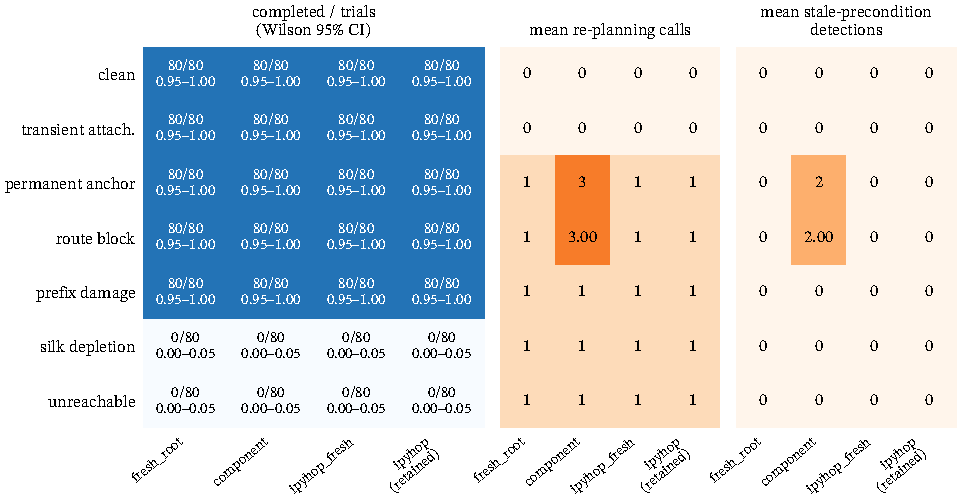
\includegraphics[width=\linewidth]{figures/recovery/rec_outcome_matrix}
\caption{Recovery benchmark outcomes by scenario and back-end, pooled over the 8 size/depth/amplitude
strata (80 trials per cell, 2,240 in total). Left: completed/trials with Wilson 95\% interval; middle:
mean re-planning calls; right: mean stale-precondition detections (cached commands rejected by the
actor). Source: \texttt{mulder\_results/recovery\_v1\_verified/trials.csv}.}
\label{fig:recovery-outcomes}
\end{figure}

\paragraph{A worked example.} Figures~\ref{fig:recovery-tree-raw}--\ref{fig:recovery-timeline} follow one
trial: 4 sectors, depth 0, 10~cm moving supports, seed 0, \texttt{permanent\_anchor}, retained IPyHOP
(\texttt{docs/research/evidence/recovery\_example}). The spider builds radii 0--2 and walks to $A_3$. At
$t=132.4$~s attachment 3 fails (leaf 31) because $A_3$ has become unavailable. \texttt{replan} keeps the
executed prefix as \texttt{old}. It backtracks to \textsc{BuildRadius}(3), whose method iterator moves
from \emph{primary} to \emph{backup}, and it un-refines the entire capture phase. The new suffix starts
with a move from the spider's actual position ($A_3\to$\,right$\to B_3$) and re-binds captures 0 and 3
from $A_3$ to $B_3$. Six queued actions are replaced by eight. The run finishes at $t=158.9$~s with 423.8~cm
of silk left. The \texttt{component} back-end, given the same event, executed the cached
\texttt{capture(0, A0, A3)} and \texttt{capture(3, A3, A2)}, had both rejected as stale, and re-planned
twice more (Figure~\ref{fig:recovery-timeline}b). Figure~\ref{fig:recovery-gallery} shows the same case
for every scenario. Route blocking at the first move re-refines almost the whole tree (48 of 53 nodes
new). Prefix damage keeps 41 old nodes and grows a \textsc{RestoreStructure} subtree. The two infeasible
scenarios exhaust the search, and the tree collapses to its root. The colour of a node records its
\emph{planning} tag only. In \texttt{prefix\_damage} the radius-0 subtree is tagged \texttt{old} although
its physical effect has been invalidated, and the observer, not the tree, is what triggers its
reconstruction (claim C20).

\begin{figure}[!htbp]
\centering
\begin{subfigure}{0.49\linewidth}\centering
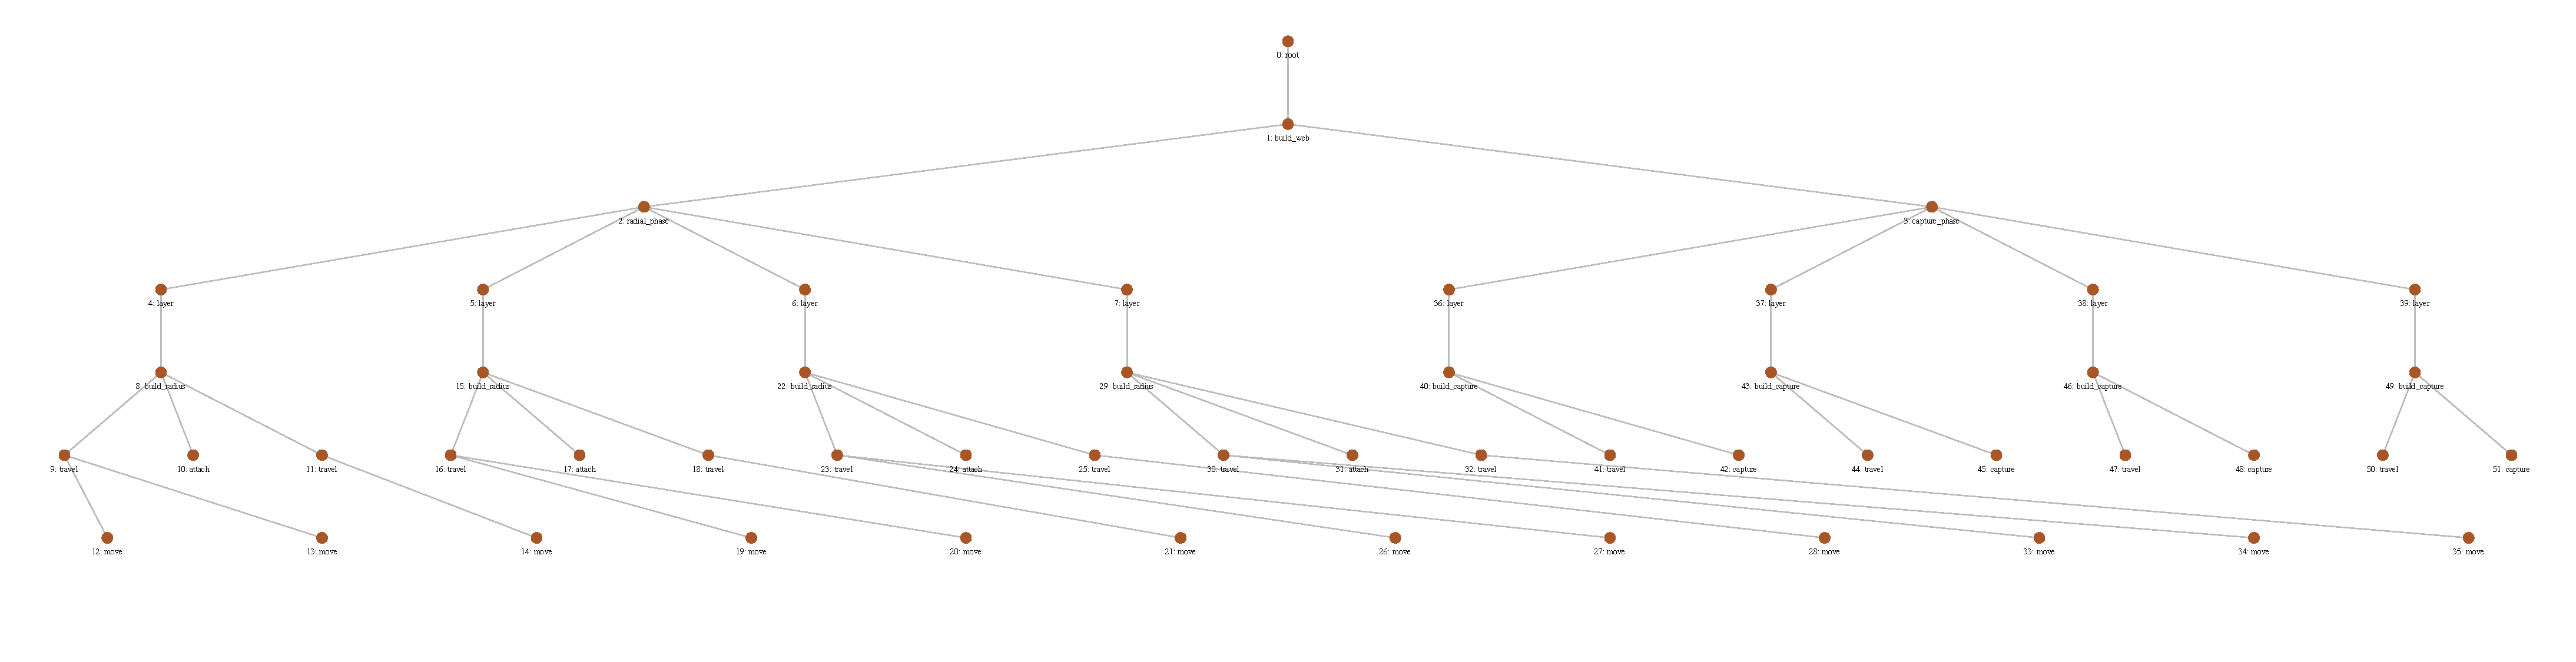
\includegraphics[width=\linewidth]{figures/recovery/tree_manuscript_initial}
\caption{initial tree (generation 1)}
\end{subfigure}\hfill
\begin{subfigure}{0.49\linewidth}\centering
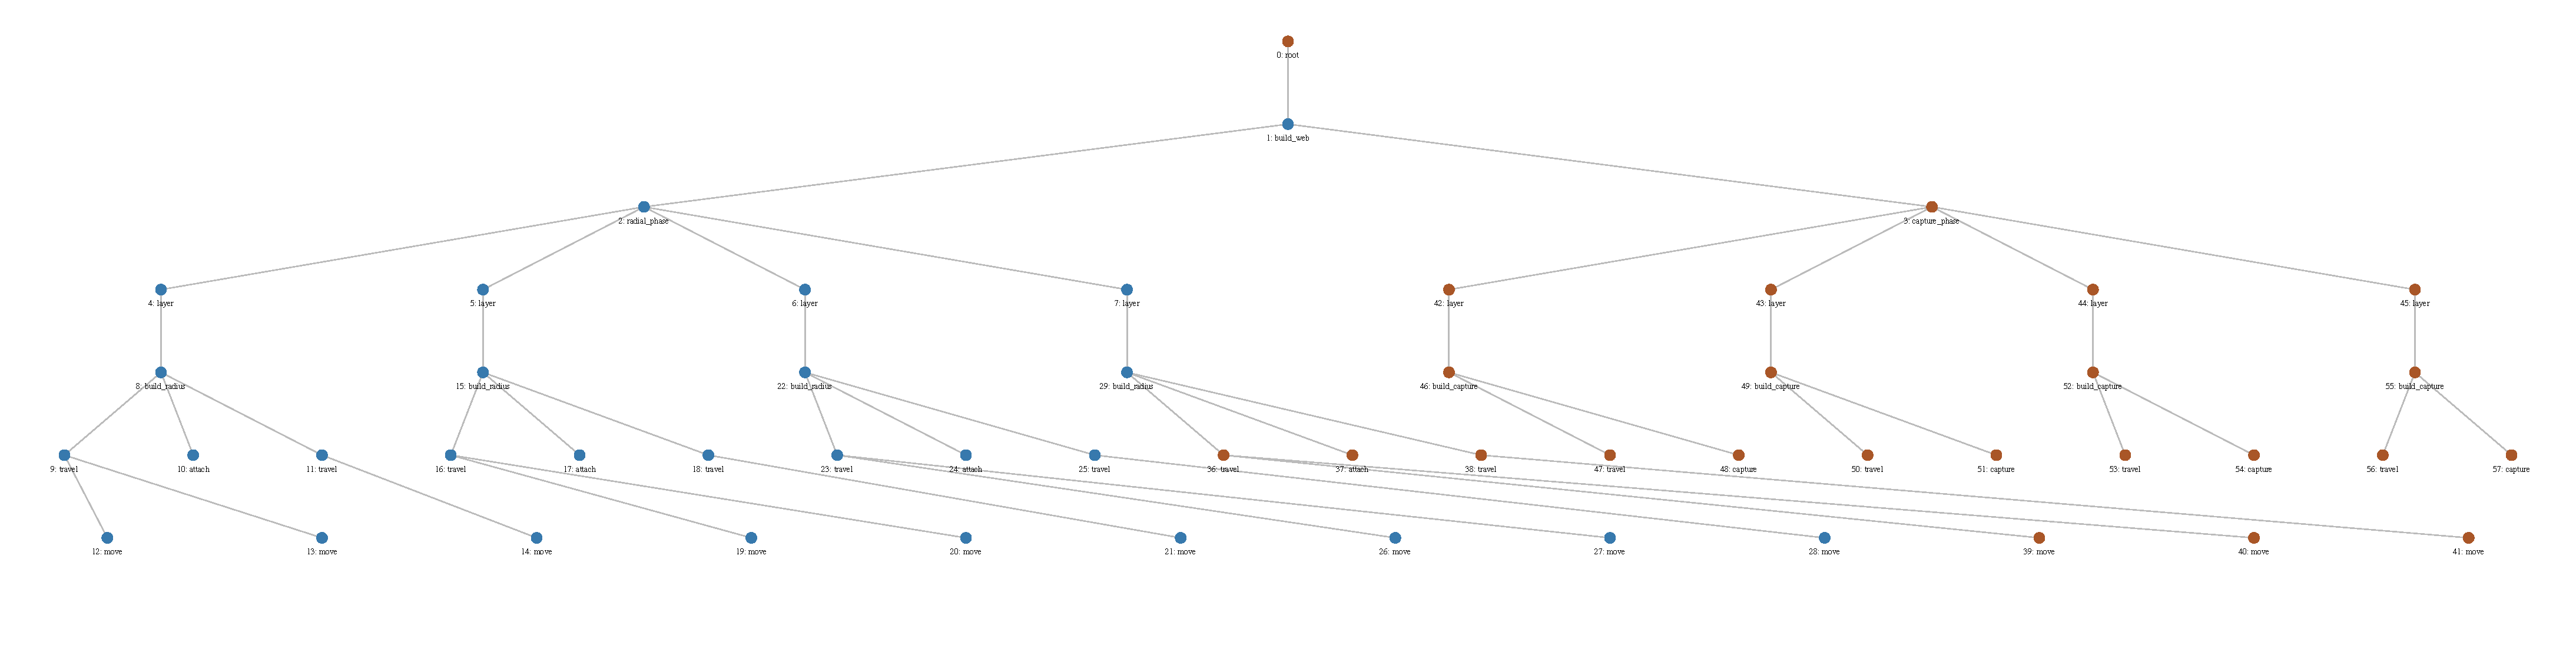
\includegraphics[width=\linewidth]{figures/recovery/tree_manuscript_replanned}
\caption{after \texttt{replan} at node 31}
\end{subfigure}
\caption{Shown for provenance only: the repository's own renderings of the recorded upstream IPyHOP solution trees for the worked
example (52 nodes each; blue = tag \texttt{old}, orange-brown = otherwise, root included). The layout is
breadth-first, so edges cross and labels are only legible when zoomed. Figure~\ref{fig:recovery-tree} is
a legible redraw of the same data. Sources:
\texttt{docs/manuscript/figures/recovery\_v1\_tree\_initial.svg},
\texttt{\ldots\_replanned.svg} (identical to \texttt{traces/case1\_permanent\_anchor\_ipyhop/tree\_\{0,1\}.svg}).}
\label{fig:recovery-tree-raw}
\end{figure}

\begin{figure}[!htbp]
\centering
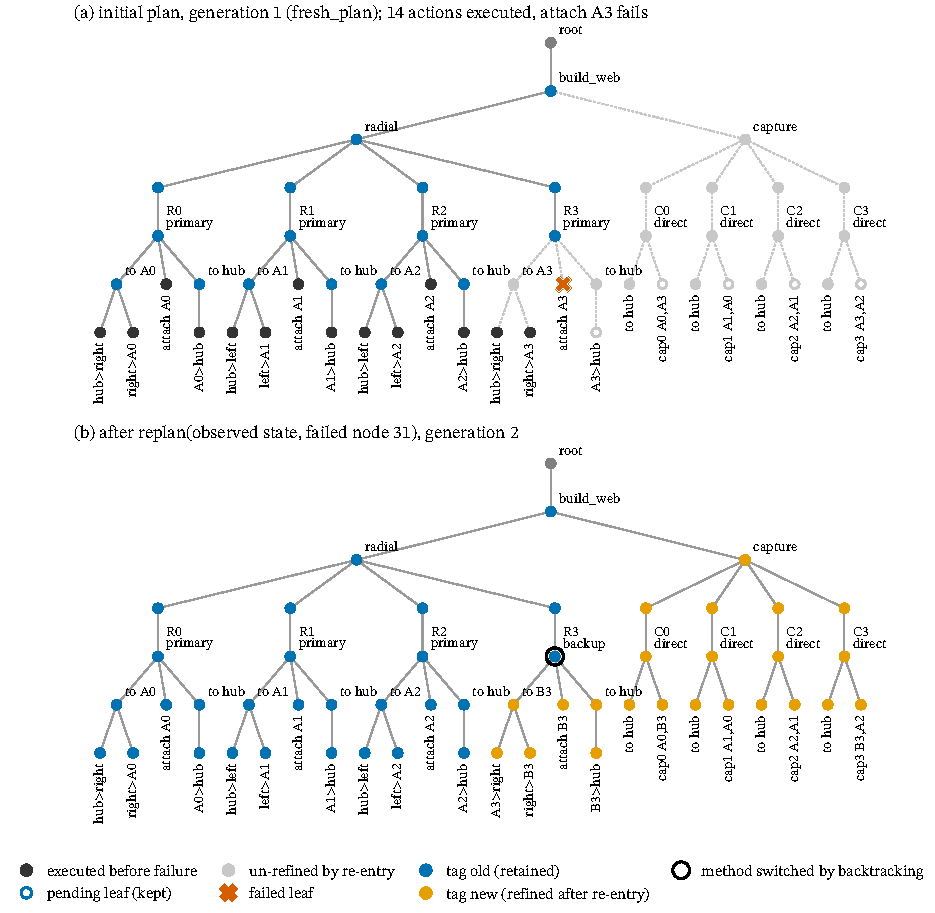
\includegraphics[width=\linewidth]{figures/recovery/tree_example_before_after}
\caption{Re-entry in the worked example, redrawn from the recorded tree snapshots. (a) Initial plan with
the 14 leaves executed before the failure (black), the failed leaf 31, \texttt{attach A3} (red cross),
and the nodes that re-entry un-refines (grey, dashed). (b) Tree returned by \texttt{replan}: retained
refinements (blue, tag \texttt{old}), new refinements (orange) and the node whose method was switched by
backtracking (ring; \textsc{BuildRadius}(3): primary$\to$backup). Leaf labels are actions
(\texttt{A3>right} = move); C$i$ = \textsc{BuildCapture}($i$) with its method. Sources:
\texttt{docs/research/evidence/recovery\_example/\{trees,events\}.json}.}
\label{fig:recovery-tree}
\end{figure}

\begin{figure}[!htbp]
\centering
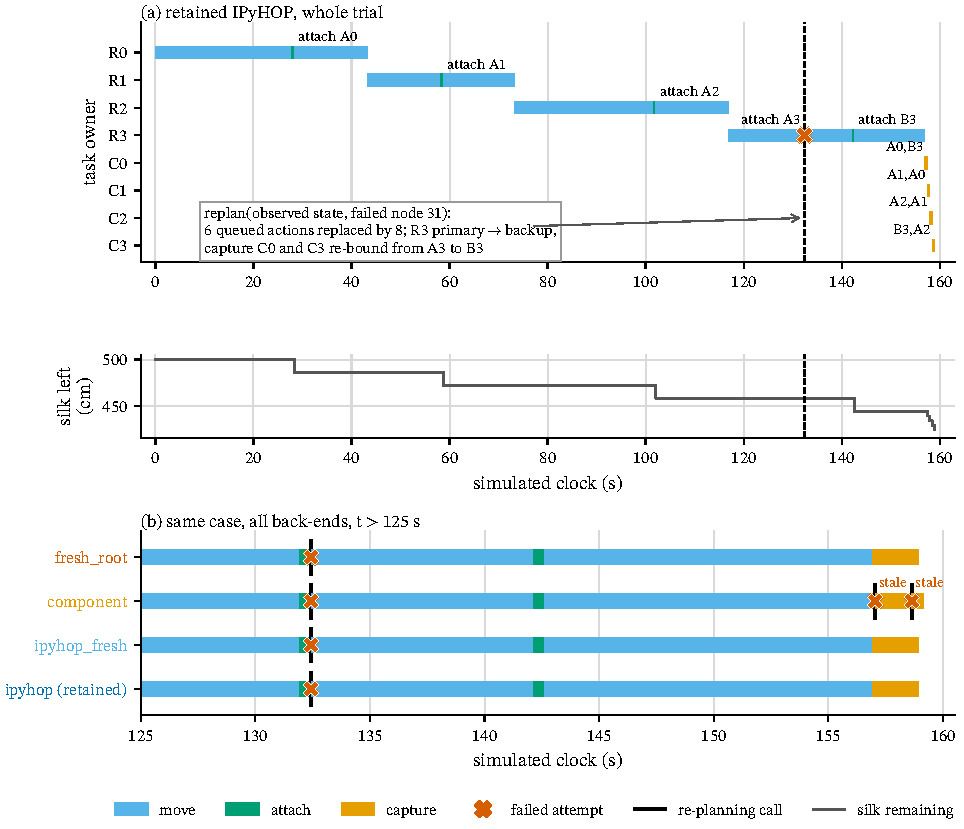
\includegraphics[width=\linewidth]{figures/recovery/rec_event_timeline}
\caption{Event ledger of the worked example. (a) Every action on the simulated clock, by task owner
(R$i$ radius, C$i$ capture sector), with the failed attempt and the re-planning call; (middle) silk
remaining. (b) The same case for all four back-ends after $t=125$~s. Only \texttt{component} meets stale
cached capture commands and re-plans twice more. Sources:
\texttt{docs/research/evidence/recovery\_example/events.json} and
\texttt{mulder\_results/recovery\_v1\_verified/traces/case1\_permanent\_anchor\_<backend>/events.json}
(one trial per back-end).}
\label{fig:recovery-timeline}
\end{figure}

\begin{figure}[!htbp]
\centering
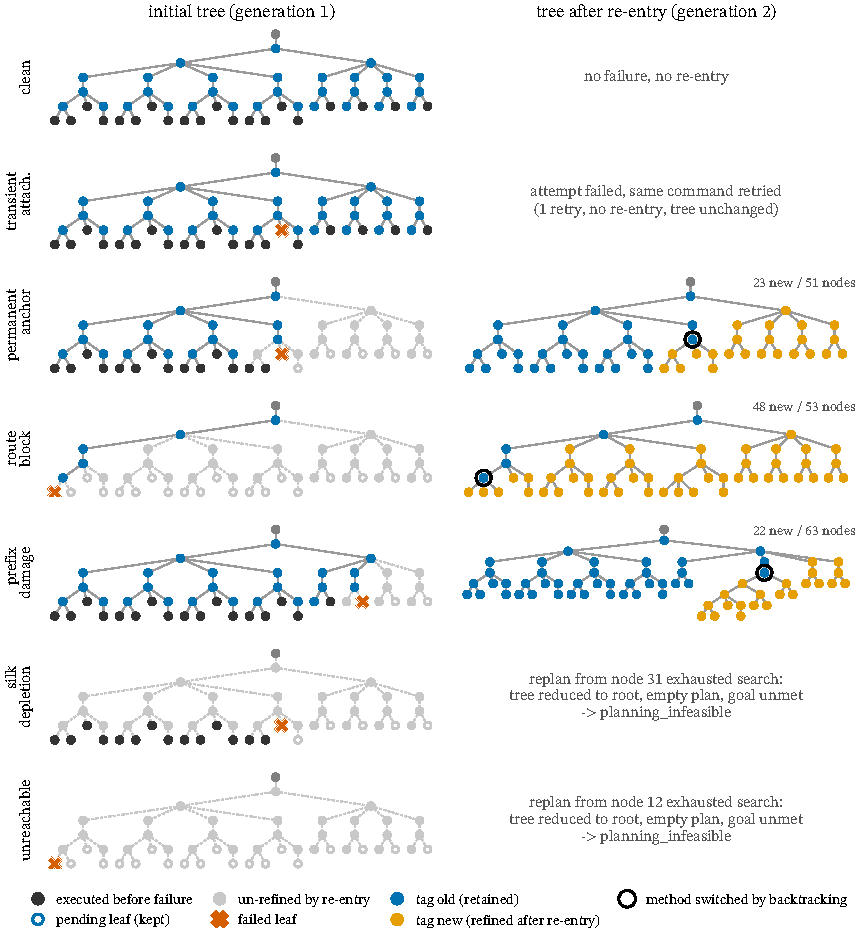
\includegraphics[width=\linewidth]{figures/recovery/tree_gallery}
\caption{Solution trees before and after re-entry, one case per scenario (4 sectors, depth 0, 10~cm,
seed 0, retained IPyHOP; colours as in Figure~\ref{fig:recovery-tree}, labels omitted). \texttt{clean}
and \texttt{transient\_attachment} never re-enter: the transient miss is retried with the same command.
\texttt{silk\_depletion} and \texttt{unreachable} exhaust the search, so the tree is reduced to its root,
the plan is empty and the trial ends \texttt{planning\_infeasible}. Sources:
\texttt{mulder\_results/recovery\_v1\_verified/traces/case1\_<scenario>\_ipyhop/\{trees,events\}.json}.}
\label{fig:recovery-gallery}
\end{figure}

\paragraph{Planning effort.} In absolute terms (Figure~\ref{fig:recovery-effort}) both IPyHOP modes
made fewer method calls than the GTPyhop DFS baselines (clean construction, pooled: 81 against 117), but
took roughly twice the planning wall time. The like-for-like comparison is retained against fresh IPyHOP
(Figure~\ref{fig:recovery-paired}). In the 8-sector, depth-2, 10~cm stratum, retention reduced method
calls by 19.6 (95\% interval $-24.8$ to $-14.4$) for \texttt{permanent\_anchor}, by 10.0 ($-11.2$ to
$-8.8$) for \texttt{route\_block} and by 38.0 for \texttt{prefix\_damage} (zero variance). It
\emph{increased} them by 11.2 (7.6 to 14.8) for \texttt{silk\_depletion}: here re-entry backtracks
through the retained tree before it establishes infeasibility. Across all 56 scenario-by-stratum cells,
method calls fell in 32, were unchanged in 16 (\texttt{clean}, \texttt{transient\_attachment}: no
re-entry) and rose in all 8 \texttt{silk\_depletion} cells. So re-entrancy does not always reduce
planning cost (claim C21). Fewer method calls also did not mean less planning time. The mean wall-time
difference was positive in 46 of the 56 cells, and its interval lay wholly above zero in 33. Examples are
$+0.91$~ms (0.24 to 1.69) for \texttt{permanent\_anchor} and $+1.58$~ms (1.26 to 1.93) for
\texttt{prefix\_damage}, even though retention made 38 fewer calls. These are millisecond measurements
that include adapter and snapshot overhead, so they describe this implementation, not the algorithm.

\begin{figure}[!htbp]
\centering
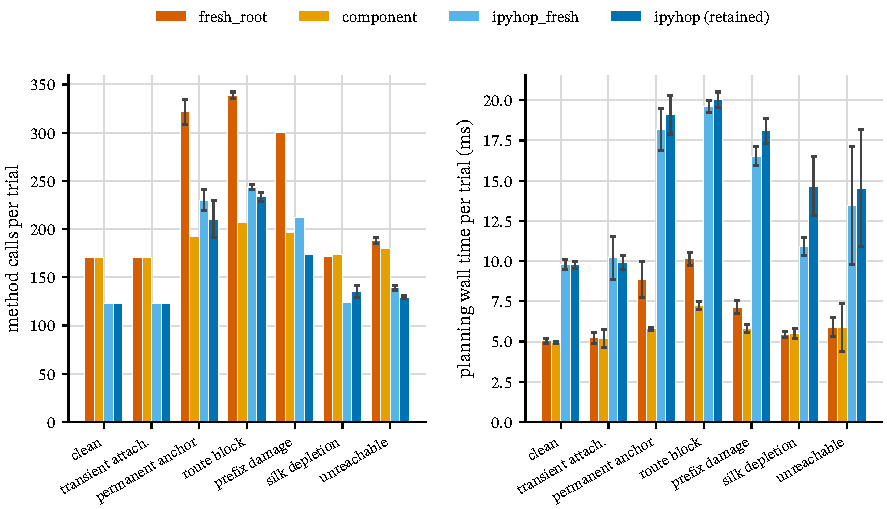
\includegraphics[width=0.85\linewidth]{figures/recovery/rec_planning_effort}
\caption{Planning effort per trial for all back-ends in the 8-sector, depth-2, 10~cm stratum (mean
$\pm$ SD over 10 seeds; GTPyhop baselines use explicit DFS backtracking). Method calls include the shared
resource guard. Planning wall time includes adapter set-up and, for IPyHOP, a tree snapshot per call.
Source: \texttt{mulder\_results/recovery\_v1\_verified/trials.csv}.}
\label{fig:recovery-effort}
\end{figure}

\begin{figure}[!htbp]
\centering
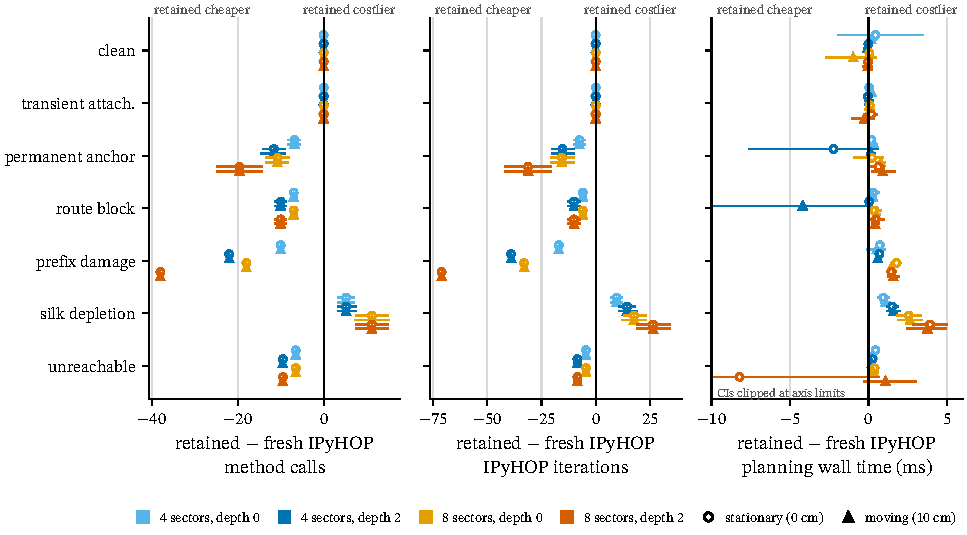
\includegraphics[width=0.9\linewidth]{figures/recovery/rec_paired_effort}
\caption{Same-engine paired contrasts, retained minus fresh IPyHOP, for every scenario and stratum
(colour: sectors and depth; marker: support amplitude). Points are means over 10 matched seeds, bars are
the repository's pointwise paired-bootstrap 95\% intervals. Failed trials are included. The wall-time
axis is clipped at $-10$~ms, which truncates three wide intervals. Negative is cheaper for retention.
Source: \texttt{mulder\_results/recovery\_v1\_verified/paired.json}.}
\label{fig:recovery-paired}
\end{figure}

\paragraph{Execution outcomes.} The back-ends' physical outcomes are identical
(Figure~\ref{fig:recovery-exec}). In all 560 matched cases, travel and silk used are the same across all
four back-ends, and the retained-minus-fresh differences in elapsed time, travel and silk are exactly
zero in all 400 completed pairs. The only elapsed-time differences belong to \texttt{component}: in 160
cases it took longer, by 0.09--0.50~s (median 0.2~s). Each stale-precondition rejection costs 0.1~s,
which accounts for the differences that are multiples of 0.1~s; we did not trace the 30 cases with other
values. No back-end
ever repeated still-valid completed work (0 unnecessary repeats in 2,240 trials).
\texttt{prefix\_damage} produced exactly one legitimate restoration per trial. Routes stayed graph-valid,
and recovery started from the observed position (claim C19). The retraced-distance measure is
owner-scoped. It is highest for \texttt{component} under \texttt{route\_block} (70.9~cm in the primary
stratum), even though total travel is the same, so it should not be read as extra walking.

\begin{figure}[!htbp]
\centering
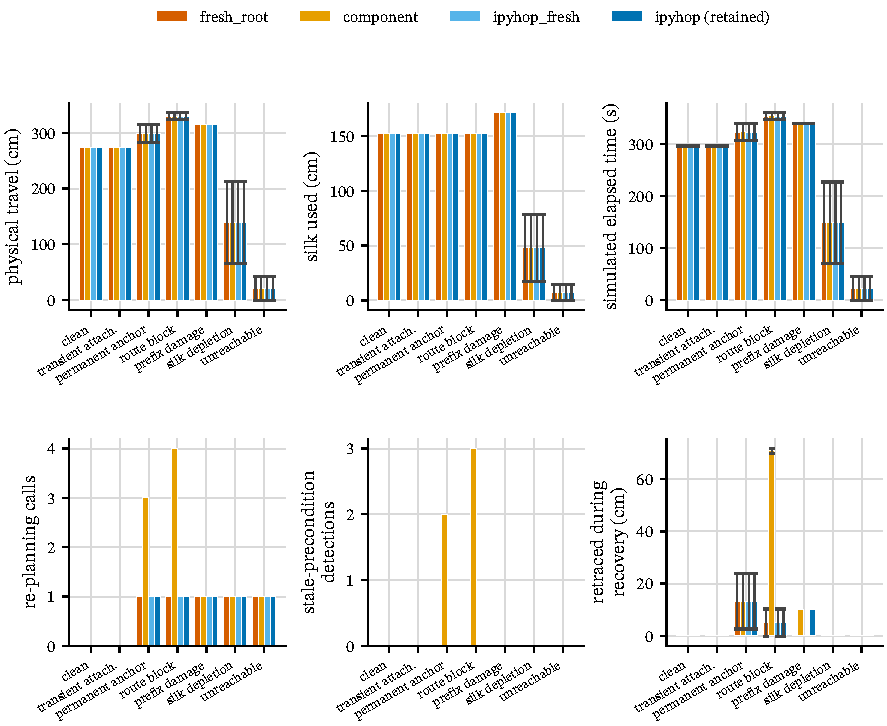
\includegraphics[width=\linewidth]{figures/recovery/rec_execution_outcomes}
\caption{Execution outcomes in the 8-sector, depth-2, 10~cm stratum (mean $\pm$ SD over 10 seeds; no bar
where SD $=0$). Travel and silk are identical for all back-ends. Infeasible scenarios stop early, which
explains their low and variable values. Source: \texttt{mulder\_results/recovery\_v1\_verified/trials.csv}.}
\label{fig:recovery-exec}
\end{figure}

% ---------------------------------------------------------------------------
\subsection{Integration into the Mulder model (v4)}
\label{sec:recovery-v4}

The Mulder moving-support model simulates the construction of a prescribed orb-web geometry on
sinusoidally shearing supports under six feedback/trigger policies (\texttt{fixed}, \texttt{local},
\texttt{filtered}, \texttt{local\_repair}, \texttt{full}, \texttt{predictive}); it is described in its
own section. Its v3 recovery is not tree re-entry. It is a fresh GTPyhop call on the failed component,
with completed-index guards and cached later components spliced on (claim C13). Version~4
(\texttt{spider\_web\_mulder/reentrant.py}) adds IPyHOP as an opt-in back-end. Historical v3 outputs and
the legacy default are unchanged.

The hierarchy becomes web $\to$ component $\to$ \textsc{PerformSegment} $\to$ \texttt{place\_segment}.
Each segment has a finite family of equivalent \emph{current-target} methods (the per-action repair
budget plus two, here 5). Each method recomputes the endpoint command from the observed clock. These are
command-refresh alternatives, not new construction strategies. Fresh IPyHOP re-plans from the root after
every failure or proactive trigger. Retained IPyHOP calls \texttt{replan} with the actual current leaf.
In both modes the whole unexecuted suffix replaces the queue, and runtime assertions reject omitted,
repeated or reordered segment indices. The legacy back-end keeps the v3 component/root scopes and the
default greedy GTPyhop strategy. The sweep (\texttt{spider\_web\_mulder/recovery\_comparison.py},
\texttt{mulder\_results/mulder\_reentrant\_v4}) has 3 back-ends $\times$ 6 policies $\times$ 10 seeds
$\times$ 2 sizes (small: 4 radii, 1 auxiliary and 1 capture turn; configured: 16/3/8) $\times$ 6 profiles
(rigid; 10~cm at 0.049~Hz; 10~cm at 0.05~Hz; one synthetic miss at segment 10; 1~s sensing lag; endpoint
execution). We counted \textbf{2,160 trials} in \texttt{trials.csv}, 720 per back-end, as the ledger
states.

\paragraph{Completion.} Figure~\ref{fig:recovery-v4-completion} gives every cell. Completion is decided by
the policy and the profile, not by the planner. Endpoint execution failed in all 360 endpoint trials. All
four retry-capable policies recovered from the single synthetic miss with every back-end and both sizes.
\texttt{local} has no retry and \texttt{fixed} fails before segment 10, so both fail that profile. The only
back-end-dependent cells are the lagged \texttt{filtered} policy, discussed below.

\begin{figure}[!htbp]
\centering
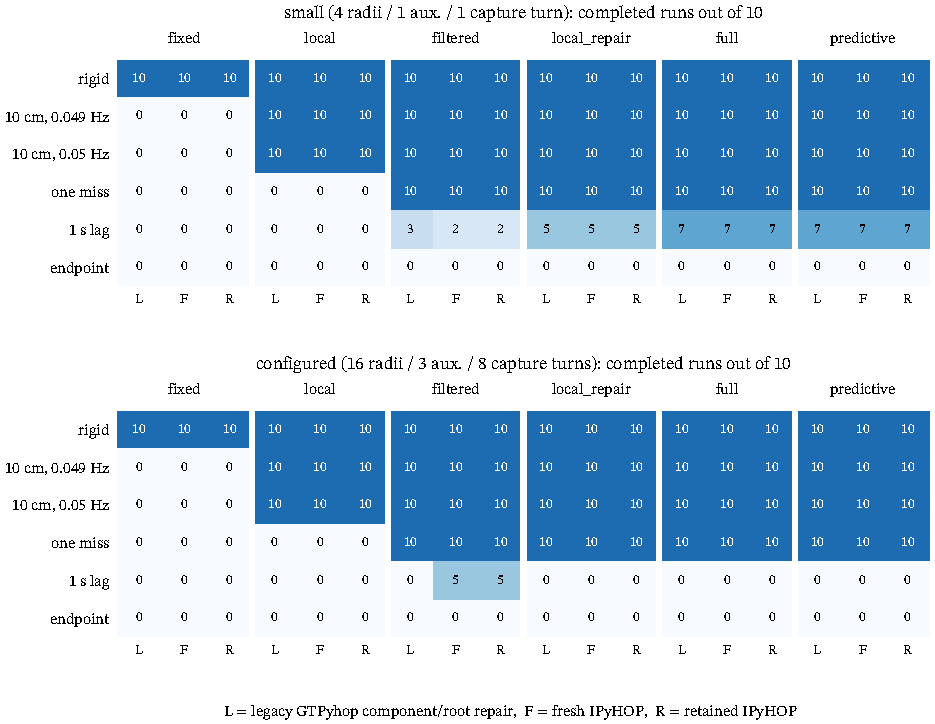
\includegraphics[width=\linewidth]{figures/recovery/v4_completion}
\caption{Mulder v4: completed runs out of 10 seeds for each profile, policy and back-end (L legacy
GTPyhop, F fresh IPyHOP, R retained IPyHOP), for both construction sizes; 2,160 trials. Source:
\texttt{mulder\_results/mulder\_reentrant\_v4/trials.csv}.}
\label{fig:recovery-v4-completion}
\end{figure}

\paragraph{Retention did not change any physical outcome (C25).} Across \textbf{all 720 matched
retained-versus-fresh IPyHOP pairs}, completion, completed actions, repairs, elapsed simulated time,
travel and the number of planning calls were exactly identical, including the failed runs
(Figure~\ref{fig:recovery-v4-pairs}). Tree retention did not improve physical outcomes in these declared
cases. Its only effect was computational. Method calls fell in 320 pairs and never rose. Planning wall
time rose in 515 pairs.

\begin{figure}[!htbp]
\centering
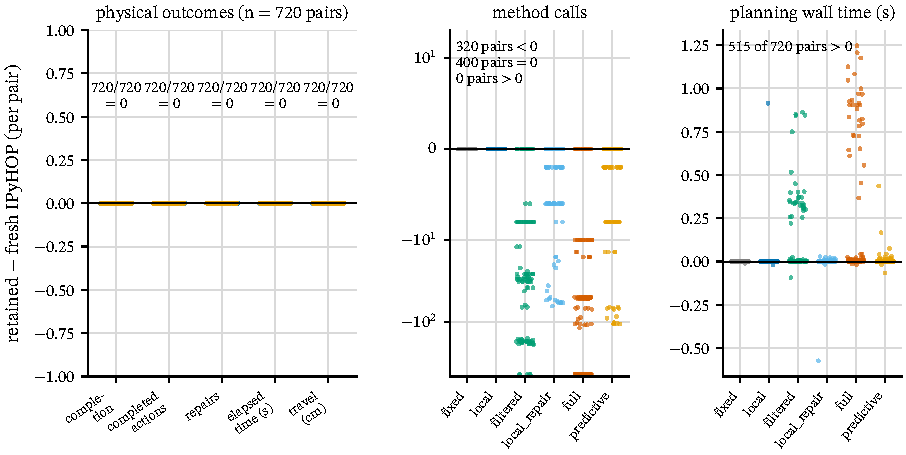
\includegraphics[width=\linewidth]{figures/recovery/v4_pair_differences}
\caption{Per-pair differences, retained minus fresh IPyHOP, in Mulder v4 ($n=720$ pairs matched on
policy, seed, size and profile; points jittered horizontally, coloured by policy). Left: all five
physical outcomes are exactly zero in every pair. Middle: method calls (symmetric-log axis). Right:
planning wall time. Source: \texttt{mulder\_results/mulder\_reentrant\_v4/trials.csv}.}
\label{fig:recovery-v4-pairs}
\end{figure}

\paragraph{Fewer method calls did not mean faster planning (C26).} At configured size, 10~cm, 0.05~Hz,
under \texttt{full} control, mean method calls were 2,095 (legacy, a different planner with fewer task
nodes), 25,966 (fresh IPyHOP) and 25,532 (retained IPyHOP). Retention therefore saved 434 calls (1.67\%;
interval $-434$ to $-434$), but mean planning wall time \emph{rose} from 1.816~s to 2.658~s, a paired
increase of 0.842~s (0.748--0.945). Without the trace-recording seed 0 the means are 1.823~s and
2.628~s, so tree recording does not explain the slowdown. Under \texttt{filtered} control the saving was
175.4 calls ($-179.2$ to $-171.4$) and the cost 0.306~s more (0.232--0.363).
Figure~\ref{fig:recovery-v4-calls} plots all 32 cells in which retention changed the call count. Calls
fell by 0.4--10.7\% in all of them, and in 30 the wall-time interval lies wholly above zero.

\begin{figure}[!htbp]
\centering
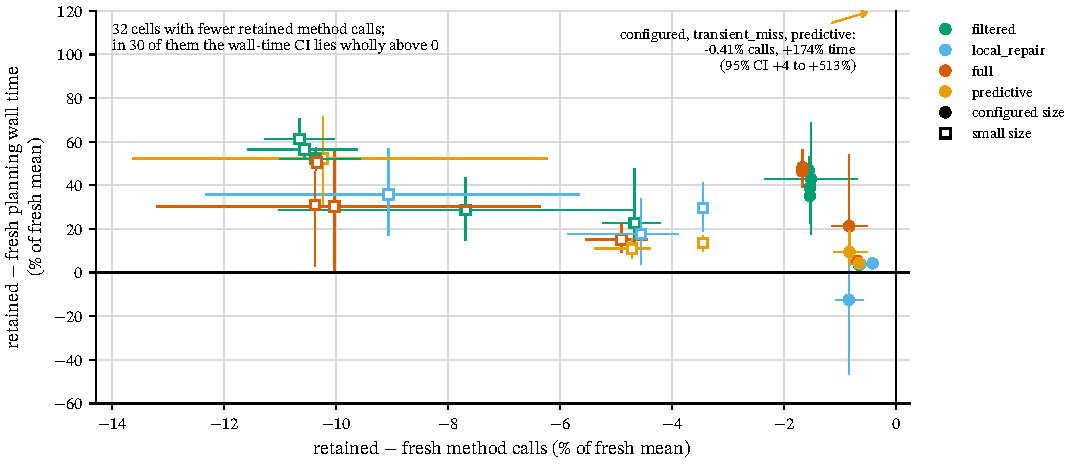
\includegraphics[width=\linewidth]{figures/recovery/v4_calls_vs_time}
\caption{Method calls against measured planning time, retained minus fresh IPyHOP, relative to the
fresh-IPyHOP mean, for the 32 size/profile/policy cells where the call count changed (10 paired seeds
each). Bars are the repository's pointwise paired-bootstrap 95\% intervals (2,000 replicates). One
off-scale cell is annotated rather than plotted. Wall time includes adapter and leaf-mapping overhead.
Sources: \texttt{mulder\_results/mulder\_reentrant\_v4/paired.json}, \texttt{trials.csv}.}
\label{fig:recovery-v4-calls}
\end{figure}

\paragraph{The lagged-completion gain is not a re-entrancy effect (C27).} With 1~s sensing lag at
configured size, \texttt{filtered} control completed 0/10 with legacy repair and 5/10 with either
IPyHOP mode (paired difference 0.5, interval 0.2--0.8). To find the cause, the repository ran 10 further
diagnostic trials with the \emph{original} GTPyhop domain and controller and changed only one thing:
the component splice was replaced by a whole-suffix refresh from the root
(\texttt{docs/research/probes/mulder\_suffix\_control.py}). This control also completed 5/10. Seed by
seed, it matched both IPyHOP modes in completion, completed actions and repairs, and in elapsed time and
travel to within $3\times10^{-13}$ (CSV versus JSON float representation;
Figure~\ref{fig:recovery-v4-lag}). It also planned faster (mean 0.556~s per run, against 0.978~s fresh
and 1.398~s retained). The improvement therefore comes from refreshing the whole suffix, not from
retained-tree re-entry. It is not universal either: at the small size, lagged \texttt{filtered}
completion fell from 3/10 (legacy) to 2/10 with either IPyHOP mode.

\begin{figure}[!htbp]
\centering
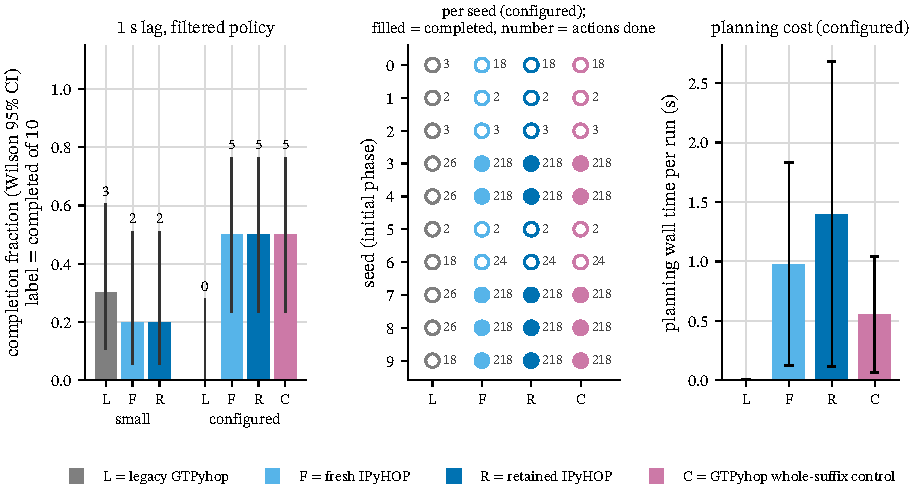
\includegraphics[width=\linewidth]{figures/recovery/v4_lag_control}
\caption{1~s sensing lag, \texttt{filtered} policy. Left: completion fraction with Wilson 95\% interval
(10 seeds per bar; C = GTPyhop whole-suffix control, configured size only). Middle: per-seed outcome at
configured size (filled = completed; number = segments completed of 218). Right: planning wall time per
run (mean $\pm$ SD over the 10 runs, failures included). Sources:
\texttt{mulder\_results/mulder\_reentrant\_v4/trials.csv},
\texttt{docs/research/evidence/mulder\_suffix\_control.json}.}
\label{fig:recovery-v4-lag}
\end{figure}

% ---------------------------------------------------------------------------
\subsection{Software verification}
\label{sec:recovery-tests}
We ran the test suites in a private clone at commit \texttt{61d18d8} (Python 3.13.3, GTPyhop 1.9.7,
NetworkX 3.6.1; the recorded study runs used Python 3.12.0 and NetworkX 3.4.2).
Table~\ref{tab:recovery-tests} lists the counts. The ledger's ``176 tests'' (C24, last reported on
2026-10-24) covers the same three directories. We observed \textbf{177 passed}, one more than the ledger
records. These tests verify software behaviour, not biology. They cover, for example, the common
recovery contract for every back-end and scenario, upstream hash pinning, prefix re-use and suffix
rebuild, the component-cache stale-suffix problem, transient retry without blacklisting, the
observed-position rule, graph-valid detours, empty-plan $\neq$ success, strategy restoration, same-engine
agreement in Mulder, and repeated re-entry with a refreshed clock.

\begin{table}[!htbp]
\centering
\caption{Tests observed passing at commit \texttt{61d18d8} (\texttt{pytest -q}, our run).}
\label{tab:recovery-tests}
\begin{tabular}{@{}lr@{}}
\toprule
Scope & Passed \\
\midrule
\texttt{spider\_web\_recovery/tests/test\_recovery.py} & 44 \\
\texttt{spider\_web\_mulder/tests/test\_reentrant.py} (v4 re-entrant integration) & 18 \\
\texttt{spider\_web\_mulder/tests} (all four files, incl.\ the 18 above) & 77 \\
\texttt{spider\_web\_htn\_updated/tests} & 56 \\
\midrule
Ledger scope: the three directories together & 177 \\
\bottomrule
\end{tabular}
\end{table}

% ---------------------------------------------------------------------------
\subsection{What is and is not supported}
\label{sec:recovery-scope}
Supported, within the stated scope:
\begin{itemize}
  \item Retained-tree recovery with the actual upstream IPyHOP handles the declared changed-anchor,
        detour, dependent-suffix and damaged-prefix cases of the authored sector domain and terminates
        correctly on the two infeasible ones (C18--C20).
  \item Splicing cached later actions after a local repair (the v3-style \texttt{component} scope)
        produces stale commitments when a repair changes a dependency. Re-planning the whole remaining
        suffix avoids them, whether from a retained tree or from the root.
  \item The new GTPyhop baselines pin full DFS backtracking (C22). The historical runs did not pin it,
        and the installed default is greedy (C15).
  \item IPyHOP is now an opt-in back-end of the actual Mulder HTN, tested in 2,160 trials (C24).
\end{itemize}
Not supported, and reported as negative results:
\begin{itemize}
  \item Retained IPyHOP did \emph{not} improve physical outcomes over fresh IPyHOP in Mulder: all 720
        pairs were identical (C25). In the sector benchmark too, physical outcomes were identical across
        back-ends.
  \item Fewer method calls did not mean faster planning: measured wall time rose in the primary Mulder
        comparisons (C26), and in most sector-benchmark cells.
  \item Re-entrancy does not always reduce planning cost: infeasible silk-depletion cases cost more
        method calls (C21).
  \item The lagged-completion gain is not unique to re-entrancy. A GTPyhop whole-suffix refresh
        reproduces it seed for seed, and at the small size IPyHOP was worse (C27).
  \item The published Run-Lazy-Refineahead evaluation is not reproduced. The actor is custom, checks only
        immediate preconditions, runs no whole-suffix simulation, and works on a different domain (C23).
  \item The IPyHOP actor integration is existing prior work applied to this domain, not a new general
        recovery algorithm (C16).
\end{itemize}
Further limits: the sector domain is authored (scaffolds, backup anchors, restoration methods, the
second routing method and the resource bound are supplied equally to all back-ends). Capture sectors are
abstract 5~cm operations. Events are logical-action triggers, not calibrated biological disturbances.
Wrapper depth adds nesting, not decisions. Mulder~v4 adds no graph, resource or damage semantics, so the
richer recovery mechanisms are tested only in the sector benchmark. Neither study measures spiders, and
neither may be pooled with the other or with the 2,280-trial Mulder~v3 study.
